% !TEX TS-program = pdflatex
% !TEX encoding = UTF-8 Unicode

% This is a simple template for a LaTeX document using the "article" class.
% See "book", "report", "letter" for other types of document.

\documentclass[11pt]{article} % use larger type; default would be 10pt

\usepackage[utf8]{inputenc} % set input encoding (not needed with XeLaTeX)
\usepackage{caption}
\usepackage{subcaption}
\usepackage{lscape} 
\usepackage{rotating}
\usepackage{longtable}
\usepackage{graphicx}
%%% Examples of Article customizations
% These packages are optional, depending whether you want the features they provide.
% See the LaTeX Companion or other references for full information.

%%% PAGE DIMENSIONS
\usepackage{geometry} % to change the page dimensions
\geometry{a4paper} % or letterpaper (US) or a5paper or....
% \geometry{margin=2in} % for example, change the margins to 2 inches all round
% \geometry{landscape} % set up the page for landscape
%   read geometry.pdf for detailed page layout information

\usepackage{graphicx} % support the \includegraphics command and options

% \usepackage[parfill]{parskip} % Activate to begin paragraphs with an empty line rather than an indent

%%% PACKAGES
\usepackage{booktabs} % for much better looking tables
\usepackage{array} % for better arrays (eg matrices) in maths
\usepackage{paralist} % very flexible & customisable lists (eg. enumerate/itemize, etc.)
\usepackage{verbatim} % adds environment for commenting out blocks of text & for better verbatim
% These packages are all incorporated in the memoir class to one degree or another...
\setlength{\textwidth}{150mm}
\setlength{\textheight}{250mm}
\setlength{\oddsidemargin}{6mm}
\setlength{\evensidemargin}{28mm}
\setlength{\topmargin}{-15mm}
%%% HEADERS & FOOTERS
\usepackage{fancyhdr} % This should be set AFTER setting up the page geometry
\pagestyle{fancy} % options: empty , plain , fancy
\renewcommand{\headrulewidth}{0pt} % customise the layout...
\lhead{Aleatorización Sesgada}\chead{}\rhead{PEC2}
\lfoot{}\cfoot{\thepage}\rfoot{}

%%% SECTION TITLE APPEARANCE
\usepackage{sectsty}
\allsectionsfont{\sffamily\mdseries\upshape} % (See the fntguide.pdf for font help)
% (This matches ConTeXt defaults)

%%% ToC (table of contents) APPEARANCE
\usepackage[nottoc,notlof,notlot]{tocbibind} % Put the bibliography in the ToC
\usepackage[titles,subfigure]{tocloft} % Alter the style of the Table of Contents
\renewcommand{\cftsecfont}{\rmfamily\mdseries\upshape}
\renewcommand{\cftsecpagefont}{\rmfamily\mdseries\upshape} % No bold!

%%% END Article customizations

%%% The "real" document content comes below...

\title{Aleatorización Sesgada}
\author{Alvarez Estarlich, Mauro \\ Requero Martín, David \\ Serrano Gómez, Enrique}
%\date{} % Activate to display a given date or no date (if empty),
         % otherwise the current date is printed 

\begin{document}
\maketitle

\section{Resumen y Comentario}

\subsection{On the use of Monte Carlo simulation, cache and splitting techniques to improve the Clarke and Wright Savings heuristics (Juan, A. et. al. (2011))}

El transporte por carretera es el principal modo de transporte de bienes y se necesitan modelos y métodos eficientes para ayudar en los procesos de toma de decisiones de este campo.\\[0.2cm]
El artículo habla sobre el Capacitated Vehicle Routing Problem (CVRP) del cual el objetivo principal es encontrar la solución (viable) de mínimo coste. Además, se introduce el algoritmo probabilístico SR-GCWS-CS, con el cual quieren probar como se pueden usar los métodos basados en simulación para mejorar heurísticos existentes.\\[0.2cm]
\textbf{El algoritmo SR-GCWS-CS}\\[0.2cm]
Combina la simulación de Monte Carlo (MCS) con el heurístico de ahorros Clarke and Wright (CWS). Además, utiliza técnicas de “Divide y vencerás” y memoria cache de soluciones obtenidas. De esta manera, puede proveer, de manera eficiente, un conjunto de soluciones pseudo-óptimas para CVRP. \\[0.2cm]
\textbf{Combinación de MCS con CWS}\\[0.2cm]
Este método asigna una probabilidad sesgada, con ruido, a cada arista en la lista de ahorros de CWS. Aristas con mayores ahorros tendrán más probabilidad de ser escogidas antes para combinarse.\\[0.2cm]
Para cada ruta generada, el mejor orden de viaje conocido entre los nodos se guarda en una especie de memoria cache. Esto se usa para mejor la calidad de generación de futuras rutas.\\[0.2cm]
El conjunto original de nodos se divide en subconjunto disjuntos y se resuelven de manera independiente para después generar la solución global.\\[0.2cm]
Este método híbrido ofrece ventajas sobre otros metaheurísticos:
\renewcommand{\labelenumi}{\alph{enumi}}
 \begin{enumerate}
   \item) Simple.
   \item) Metodología flexible y robusta.
   \item) Buen rendimiento generando soluciones.
   \item) No requiere ajustes de alta precisión.
   \item) Se puede ejecutar en paralelo.
 \end{enumerate}

\textbf{Valoración}\\[0.2cm]
Es un artículo bien estructurado ya que responden a la mayoría de las preguntas que alguien se podría hacer al leerlo: Qué problema hay, en que consiste, como se ha solucionado y que métodos se han utilizado anteriormente, como lo van a solucionar ellos y por qué lo hacen así, etc.\\[0.2cm]
Aparte de la estructura, las explicaciones están bien hechas, dando contexto a cada nuevo concepto/término para utilizarlo más adelante. Además, da referencias para que el lector profundice si lo desea y es sencillo de entender. Hubiera sido interesante que cogieran una instancia pequeña como ejemplo y que mostraran como cambian las rutas en cada optimización añadida (CWS +MCS, CWS + MCS + Hash map, CWS + MCS + Hash map + Split ). 

\subsection{The SR-GCWS hybrid algorithm for solving the capacitated vehicle routing problem. (Juan, A. et. al. (2010))}

El artículo presenta un nuevo planteamiento para encontrar soluciones al “capacitated vehicle routing problem” (CVRP). Para ello introducen el concepto de Clarke and Wright Savings (CWS), que es usado para asignar una puntuación a cada arista en función del “ahorro” que supone seleccionarlo para moverse de un nodo a otro, siempre y cuando no se violen las reglas establecidas por el problema. También se añade la técnica de Monte Carlo simulation (MCS) ya que se ha visto que resulta muy útil a la hora de resolver problemas complejos mediante el uso de números aleatorios y distribuciones estadísticas.\\[0.2cm]
Poniéndolo todo junto, para cada paso en el que se deba seleccionar una nueva arista, primero se seleccionan aquellas que tengan un mayor “ahorro” y a cada una de ellas se le asigna una probabilidad de ser seleccionada (mayor probabilidad a los que presenten un “ahorro” mayor). La probabilidad que se asignará vendrá determinada por una distribución (cuasi-) geométrica, también seleccionada de un conjunto de distribuciones posibles. En concreto, el punto clave es la generación de cientos de soluciones posibles, cada una de ellas generada a partir de una versión aleatorizada de la solución obtenida por CWS. Con todo ello, se consigue un algoritmo altamente explorativo que es capaz de mejorar los resultados obtenidos por los algoritmos más vanguardistas, dentro de un periodo de tiempo aceptable.\\[0.2cm]

\textbf{Valoración}\\[0.2cm]

El artículo plantea un algoritmo con claras ventajas frente a los algoritmos clásicos de optimización: es sencillo tanto en cuanto a la complejidad de programación como a las técnicas y conceptos que lo fundamentan, además no requiere de “tunning” de parámetros para obtener mejores resultados, por lo que se acorta el tiempo de experimentación para llegar a una solución subóptima pero aceptable cuando se compara con los mejores resultados obtenidos hasta la fecha. En cuanto a la redacción y la forma de presentar los diferentes conceptos, utilizando un lenguaje fácilmente comprensible, evitando un gran número de siglas y acrónimos, hace que la lectura no sea pesada y que el lector sea capaz de comprender los principales conceptos e ideas que se quieren transmitir. Queda por explorar el potencial de adaptación de esta solución para otros problemas de otros ámbitos.

\clearpage

\subsection{Biased Randomization of Heuristics using Skewed Probability Distributions: a survey and some applications (Grasas, A. et. al. (2017))}

La aleatorización sesgada (BRP) se platea como una solución al problema de obtener algoritmos más exploratorios que permitan obtener soluciones a lo largo de todo el dominio del problema, fuera del intervalo situado en torno a un óptimo local. Se puede implementar empleando funciones empíricas o a través del uso de uso de distribuciones de probabilidad sesgadas. El primer caso se basa en una función sesgada con un criterio que asigna un peso a cada candidato, a partir de los cuales se genera una distribución de probabilidad empírica. Sin embargo, el segundo caso presenta dos ventajas fundamentales: las distribuciones de probabilidad teóricas suelen ser función de un único parámetro fácilmente definible y se disponen de fórmulas analíticas para la obtención sus valores, que son más eficientes a nivel computacional al evitar el uso de bucles. La variación de dicho parámetro a partir de sus dos valores extremos permite obtener una selección más aleatoria o más sesgada. Empleando paralelización se pueden obtener numerosas soluciones candidato, lo cual resulta beneficioso para aplicaciones en las que le tiempo es un factor crítico. Se han implementado de forma experimental en cinco problemas de optimización con heurísticas constructivas (VRP, ARP, PFSP, UFLP, y 2DSPP). Se obtienen mejores resultados a mayor tiempo de ejecución y mayor número de agentes en paralelo. Además, se observa una mejora en los resultados frente a la heurística original, y en comparación con la aleatorización uniforme, donde se obtiene un resultado bastante deficiente en la mayoría de casos. \\[0.2cm]

\textbf{Valoración}\\[0.2cm]

El artículo expone de un método para evitar que en el proceso de selección aleatoria empleado en la elección de soluciones candidato se descarten soluciones plenamente válidas. Se explican dos formas de introducción de sesgo en BRPs: con distribuciones empíricas o con distribuciones de probabilidad teórica, lo que permite al lector entender las principales diferencias entre ambos procedimientos a través de distintos casos particulares, exponiéndose las ventajas de cada caso. Posteriormente a través de cinco problemas de optimización combinatoria se presentan de forma cuantitativa las ventajas anteriormente anunciadas. Se muestra la sensibilidad de la respuesta de cada problema individual ante los distintos parámetros de entrada, una comparación de BRP con otros procedimientos. Esto proporciona una dimensión práctica a través de ejemplos a la exhaustiva introducción teórica anterior. Gracias a esto cualquier lector independientemente de su trasfondo es capaz de entender e interpretar mejoras del procedimiento expuesto en el artículo.

\clearpage

{\fontsize{50}{60}\selectfont Diseño y desarrollo de un algoritmo de busqueda randomizada y heuristica CWS aplicada al VRP}

\renewcommand{\labelenumi}{\arabic{enumi}}
 \begin{enumerate}
   \item) \textbf{Introducción}\\[0.2cm]
El problema del rutaje de vehiculos (VRP de sus siglas en inglés) se centra en la busqueda del mejor conjunto de rutas por las que guiar a una flota de vehiculos de mercancias cuyo deber es abastecer a los clientes. Pero el problema puede ser planteado con diferentes grados de complejidad en funcion de las restricciones y detalles que se quieran considerar con tal de asemejar el sistema cada vez mas al mundo real. Las principales restricciones que se aplican al VRP se basan en:
   \begin{itemize}
       \item El uso de vehiculos con una capacidad finita en cuanto al transporte de mercancias.
       \item Que los vehiculos no pueden visitar dos veces un mismo cliente en su ruta de reparto.
       \item La presencia de un almacen desde del que todos los vehiculos salen y al que deben volver tras el reparto.
   \end{itemize} 
El VRP tiene un gran interes tanto por los beneficios económicos que puede reportar, asi como por los beneficios ecológicos que se pueden deducir del mismo.
   \item) \textbf{Revisión de la literatura}\\[0.2cm]
Para el desarrollo de nuestro algoritmo nos hemos basado en la revision de tres articulos: Juan, A. et. al. (2010) (1), Juan, A. et. al. (2011) (2) y Grasas, A. et. al. (2017) (3).\\
En el primer trabajo (1) demuestra como el uso de Clarke and Wright Savings (CWS) y simulaciones de Monte Carlo (MCS) favorecen la busqueda de soluciones con un menor "coste" y además se introduce el uso de funciones (cuasi-) geométricas para la asignación de probabilidades a los candidatos a mejor ruta. Con este enfoque se consigue que el mejor canidato pueda o no ser elegido, ya que se le asigna una probabilidad (mas elevada en funcion de la calidad de la solución) para que sea o no seleccionado.\\
En el segundo articulo (2) del mismo autor, a parte de la técnicas descritas anteriormente se añade el concepto de "splitting", basado en el principio de "divide y vencerás", por el cual se subdivide el conjunto de nodos en subgrupos para ser procesados de manera independiente y después unir las diferentes subsoluciones obtenidas en una solución única. Grácias a este planteamiento se consigue obtener soluciones donde las rutas se cruzan con menor frecuencia, es simple y permite ser ejecutado en paralelo.\\
En el articulo más reciente (3), se plantea el uso de la aleatorización sesgada como medida para obtener un algoritmo más explorativo, permitiendo obtener soluciones a lo largo de todo el dominio del problema. Para ello se plantean dos maneras de obtener distribuciones de probabilidad sesgadas, la primera basada en la obtención empirica y la segunda (y preferida) la basada en distribuciones teóricas generadas a partir de funciones matemáticas. Esta segunda opción es más rápida a nivel computacional y configurable a partir de los parametros que definen la función de distribución.

\clearpage

   \item) \textbf{Algoritmo desarrollado}\\[0.2cm]
A partir del algoritmo \textit{Clarke and Wright Savings} (CWS) hemos añadido 3 métodos que pueden ser independientes y combinados unos con otros, para mejorar la solución inicial que nos proporciona el algoritmo básico.
\begin{itemize}
\item Inicio sesgado.
\item Método de aprendizaje utilizando una memoria de rutas.
\item Método “Divide y vencerás”.
\end{itemize}
El algoritmo básico tiene 3 fases:
\renewcommand{\labelenumii}{\arabic{enumii}}
\begin{enumerate}
\item Construir las aristas entre los nodos, calculando un coste asociado al movimiento entre nodos, este coste se usa como concepto de ahorro. Se genera una lista ordenada de las aristas que suponen mayor ahorro a menos ahorro.
\item Construir una solución inicial con rutas desde el nodo inicial al nodo destino, solución que no es eficiente, pero es el punto de partida para ejecutar el siguiente paso.
\item Se itera la lista de aristas creada y se comprueba si es factible fusionar las rutas que hay desde el nodo inicial a cada nodo en los extremos de la arista. Al fusionar las rutas se consigue ahorrar costes y se empieza intentando fusionar las rutas mas costosas (que producen más ahorro).
\end{enumerate}

En este algoritmo básico aplicamos \textbf{inicio sesgado} a la lista de ahorro. Hay dos maneras de hacerlo:
\begin{enumerate}
\item El orden de la lista de ahorro es completamente aleatorio. Cada arista tiene la misma probabilidad de ser analizada y fusionada la ruta de sus nodos primero.
A este caso se le puede limitar la aleatoriedad limitando cuantas aristas tiene en cuenta. Por ejemplo, la elección de aristas es completamente aleatoria pero solo entre las 10 aristas que suponen mayor ahorro.
\item El orden de la lista de ahorro es aleatorio con una probabilidad sesgada. Esto significa que las aristas con mayor ahorro tendrán mas probabilidad de ser elegidas primero.
Podemos modificar cuanto sesgo queremos utilizar con un valor Beta. Utilizando una Beta pequeña el sesgo para elegir aristas de mayor ahorro es menor y con una Beta grande el sesgo es mayor y la elección de aristas se asemeja al algoritmo básico.
\end{enumerate}
Nosotros hemos utilizado el segundo método basándonos en la literatura investigada. El código que nos modificaba la lista de ahorro según el valor Beta es el siguiente:

\begin{figure}[h]
\centering
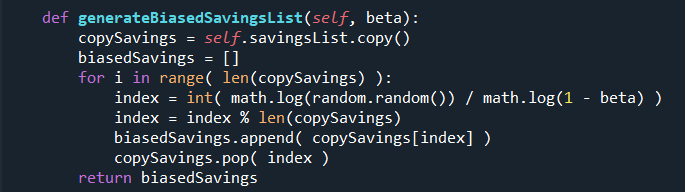
\includegraphics[width=0.8\linewidth, height=3.5cm]{generateBiasedSavingList.png} 
\label{fig:subim1}
\end{figure}

Como existe un componente aleatorio, la ejecución de este método ha de ser realizada varias veces para evitar que encontremos una anomalía estadística y que los resultados no sean fiables. Cuantas más veces iteramos las posibles anomalías desaparecen y tenemos un resultado más fiable que no depende de la “suerte” que tengamos con las probabilidades. \\

El \textbf{método de aprendizaje} mediante la cache de rutas se basa en la idea de que en cada iteración se generan rutas distintas con diferente coste (debido al inicio sesgado que utilizamos). \\

Si mantenemos un mapa con las mejores rutas encontradas para determinado conjunto de nodos, podemos mejorar el coste de la solución final encontrada comparando las rutas de la solución con las mejores rutas encontradas. \\

Por ejemplo, quizás nuestra solución final ha encontrado una ruta que implica a los nodos 0,1,2,3,4 en el orden: 0-2-3-4-1. Como hemos guardado la mejor ruta encontrada para cada conjunto de nodos, comprobamos si hay alguna manera de recorrer esos nodos con menor coste, y encontramos que la ruta 0-3-2-1-4 es más “barata” de hacer. Así que sustituiríamos la ruta final de la solución con otra mejor.\\

El código con el que hacemos esta comprobación es el siguiente:

\begin{figure}[h]
\centering
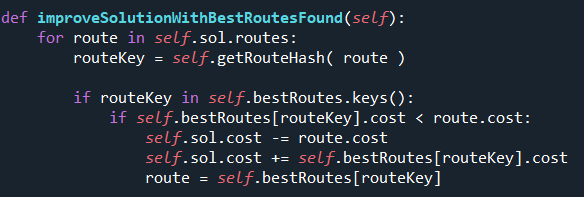
\includegraphics[width=0.8\linewidth, height=4cm]{improveSolutionWithBestRoutesFound.png} 
\label{fig:subim1}
\end{figure}

Y la actualización del mapa con rutas mejores así:

\begin{figure}[h]
\centering
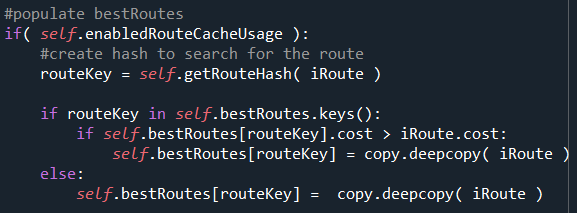
\includegraphics[width=0.8\linewidth, height=4cm]{routeHashUpdate.png} 
\label{fig:subim1}
\end{figure}

El último método que hemos aplicado es el de \textbf{“Divide y vencerás”}. Este método se basa en la división del problema inicial en subproblemas más pequeños de manera que se pueden calcular soluciones independientes que pueden mejorar las rutas encontradas. Estas soluciones una vez encontradas son juntadas y nos otorgan una solución final al problema.\\

En nuestro caso, la división del problema se hace mediante la localización de los nodos en el espacio. Cada nodo tiene unas coordenadas X e Y de manera que dividimos los nodos por su posición en el mapa.\\

\clearpage

Hemos utilizado cuatro maneras diferentes para dividir los nodos:
 \begin{enumerate}
\item Nodos por encima y por debajo de la coordenada Y(0). Genera 2 subgrupos de nodos.
\item Nodos a la derecha o izquierda de la coordenada X(0). Genera 2 subgrupos de nodos.
\item Nodos en cada uno de los 4 cuadrantes del eje de coordenadas. Genera 4 subgrupos de nodos.
\item Nodos en cada uno de los 4 cuadrantes divididos por la diagonal. Genera 8 subgrupos de nodos.
\end{enumerate}

Este método puede funcionar mejor o peor dependiendo de las características de la red. Por ejemplo, si todos los nodos están por debajo de Y(0) y utilizamos el primer enfoque, solo generaremos un subgrupo de nodos.\\
Además, hay que tener en cuenta que no siempre la división del problema nos otorgara mejores soluciones.\\

El código para dividir el mapa de nodos y encontrar soluciones independientes es el siguiente:

\begin{figure}[h]
\centering
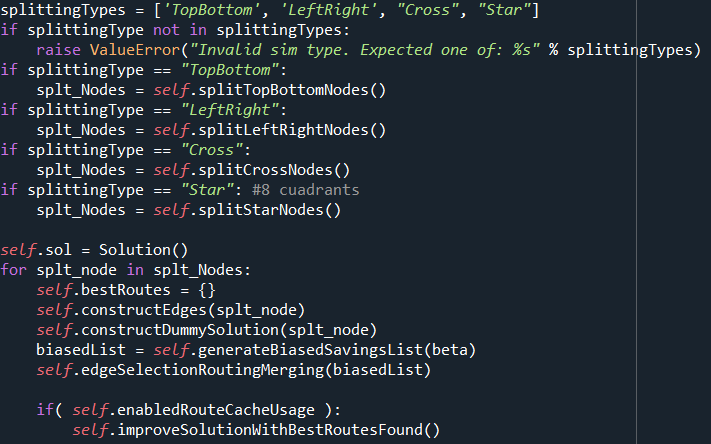
\includegraphics[width=0.8\linewidth, height=8cm]{splittingCode.png} 
\label{fig:subim1}
\end{figure}

Por último, estos 3 métodos pueden combinarse entre ellos para conseguir una mejor solución explotando las posibilidades que nos ofrece cada uno. Hemos hecho diversas pruebas combinando los 3 métodos que aparecen en el siguiente apartado.

\clearpage

   \item) \textbf{Experimento computacional y análisis de resultados}\\[0.2cm]

\begin{landscape}
\begin{table}[p]
\centering
\begin{small}
\caption{Tabla de los resultados obtenidos con $\beta = 0.3$}
\begin{tabular}{ccccccccccccc}
\toprule
\multicolumn{1}{p{1cm}}{\centering Instance} 
&  \multicolumn{1}{p{1.2cm}}{\centering Capacity} 
&  \multicolumn{1}{p{1cm}}{\centering Original\\(a)} 
&  \multicolumn{1}{p{1cm}}{\centering Random\\(b)} 
&    \multicolumn{1}{p{1.8cm}}{\centering   RandomRCU\\(c) }
&    \multicolumn{1}{p{1.5cm}}{\centering   TopBottom \\(d) }
&    \multicolumn{1}{p{1.5cm}}{\centering   LeftRight \\(e) }
&     \multicolumn{1}{p{1cm}}{\centering      Cross \\(f)}
&    \multicolumn{1}{p{1cm}}{\centering        Star \\(g) }
&   \multicolumn{1}{p{2.4cm}}{\centering  TopBottomRCU \\(h)} 
&   \multicolumn{1}{p{2cm}}{\centering LeftRightRCU \\(i) }
&    \multicolumn{1}{p{1.5cm}}{\centering    CrossRCU \\(j) }
&     \multicolumn{1}{p{1cm}}{\centering    StarRCU \\(k) }\\
\midrule
A-n32-k5&100&843.69&798.07&800.61&849.03&833.15&844.76&925.27&843.32&822.34&848.84&930.0 \\
A-n38-k5&100&768.13&766.22&764.94&761.49&810.13&838.56&908.61&771.78&809.7&849.67&905.64 \\
A-n45-k7&100&1199.98&1165.19&1159.74&1187.42&1176.15&1192.01&1345.2&1186.47&1158.05&1190.75&1350.31 \\
A-n55-k9&100&1099.84&1098.92&1095.89&1136.43&1127.77&1168.76&1289.97&1144.56&1123.09&1166.09&1287.33 \\
A-n60-k9&100&1421.88&1372.63&1367.65&1452.57&1384.94&1456.78&1555.21&1444.18&1387.16&1467.48&1557.94 \\
A-n61-k9&100&1102.23&1059.62&1053.23&1117.3&1103.73&1135.18&1239.34&1121.08&1104.48&1129.46&1244.4 \\
A-n65-k9&100&1239.42&1197.49&1212.0&1252.95&1267.87&1289.8&1422.04&1263.03&1256.06&1290.57&1429.4 \\
A-n80-k10&100&1860.94&1804.88&1809.11&1873.87&1883.98&1971.95&2001.05&1878.78&1874.35&1965.89&2024.23 \\
B-n50-k7&100&748.8&748.26&744.34&762.06&761.07&790.96&990.0&759.59&759.73&788.86&984.17 \\
B-n52-k7&100&764.9&760.28&758.71&849.92&764.79&895.64&962.88&849.62&765.59&890.12&962.39 \\
B-n57-k9&100&1653.42&1638.57&1638.66&1617.44&1739.88&1658.24&1745.7&1639.58&1740.46&1737.77&1747.41 \\
B-n78-k10&100&1264.56&1264.16&1256.04&1276.04&1294.83&1310.33&1358.34&1271.03&1293.09&1306.88&1349.95 \\
E-n22-k4&6000&388.77&387.54&385.29&388.15&425.2&446.57&527.86&388.92&419.22&437.36&527.41 \\
E-n30-k3&4500&534.45&506.55&505.01&560.42&512.22&564.89&703.4&558.5&507.93&562.1&706.45 \\
E-n33-k4&8000&843.1&842.8&843.1&843.1&976.88&977.47&1030.5&842.8&965.0&976.01&1030.96 \\
E-n51-k5&160&584.64&555.8&554.17&576.88&579.25&594.11&708.2&572.87&576.56&606.26&689.49 \\
E-n76-k10&140&907.39&869.11&859.23&883.93&888.67&913.82&1056.45&891.83&890.67&916.69&1059.52 \\
E-n76-k14&100&1054.6&1052.33&1048.42&1078.14&1064.23&1105.75&1186.02&1083.54&1062.74&1102.32&1180.91 \\
E-n76-k7&220&738.13&731.52&723.82&749.23&755.71&775.59&844.94&759.07&753.22&789.87&831.57 \\
F-n135-k7&2210&1219.32&1211.2&1197.58&1264.63&1234.83&1270.17&1381.23&1248.32&1221.7&1280.48&1364.35 \\
F-n45-k4&2010&739.02&729.25&727.75&848.45&735.48&860.01&1064.25&851.21&735.21&872.6&1058.38 \\
F-n72-k4&30000&256.19&255.63&254.87&256.89&312.87&314.08&343.76&255.82&313.74&312.89&342.69 \\
M-n101-k10&200&833.51&831.08&825.34&836.02&930.41&952.53&1042.61&842.35&931.03&953.46&1045.53 \\
M-n121-k7&200&1068.14&1058.61&1057.76&1169.17&1070.05&1179.57&1258.6&1172.0&1066.4&1181.41&1264.19 \\ 
P-n101-k4&400&765.38&733.23&733.23&733.22&736.48&772.76&923.17&734.49&744.33&772.3&922.69 \\
P-n22-k8&3000&590.62&588.79&588.79&607.92&632.2&654.55&692.64&608.52&632.2&654.55&693.37 \\
P-n40-k5&140&518.37&483.96&485.68&501.31&509.17&531.29&656.94&487.17&514.68&523.62&635.38 \\
P-n50-k10&100&739.84&715.32&712.77&730.16&730.9&774.14&842.97&742.15&737.09&767.21&825.01 \\
P-n55-k15&70&978.07&961.64&958.73&995.03&983.0&1016.4&1129.99&990.36&979.49&1009.09&1120.39 \\ 
P-n65-k10&130&851.67&816.89&813.57&837.81&840.14&892.02&984.08&840.93&835.08&879.16&997.82 \\
P-n70-k10&135&896.86&856.02&853.62&887.51&873.54&919.75&1030.52&887.18&873.45&926.82&1056.35 \\
P-n76-k4&350&688.34&636.76&640.95&656.41&645.67&680.59&859.84&652.7&656.47&670.41&864.81 \\
P-n76-k5&280&709.38&674.47&673.98&700.73&692.28&726.77&855.59&699.46&684.75&723.36&853.03 \\
\bottomrule
\end{tabular}
\end{small}
\end{table}%

\begin{table}[p]
\centering
\begin{small}
\caption{(Continuación) Tabla de los resultados obtenidos con $\beta = 0.3$}
\begin{tabular}{ccccccccccc}
\toprule
Instance & gap1 (b)-(a) &          gap2 (c)-(a) &       gap3 (d)-(a) &       gap4 (e)-(a) &       gap5 (f)-(a) &       gap6 (g)-(a) &       gap7 (h)-(a) &       gap8 (i)-(a) &       gap9 (j)-(a) &      gap10 (k)-(a) \\
\midrule
A-n32-k5&-5.41&-5.11&0.63&-1.25&0.13&9.67&-0.04&-2.53&0.61&10.23 \\
A-n38-k5&-0.25&-0.42&-0.86&5.47&9.17&18.29&0.47&5.41&10.62&17.9 \\
A-n45-k7&-2.9&-3.35&-1.05&-1.99&-0.66&12.1&-1.13&-3.49&-0.77&12.53 \\
A-n55-k9&-0.08&-0.36&3.33&2.54&6.27&17.29&4.07&2.11&6.02&17.05 \\ 
A-n60-k9&-3.46&-3.81&2.16&-2.6&2.45&9.38&1.57&-2.44&3.21&9.57 \\
A-n61-k9&-3.87&-4.45&1.37&0.14&2.99&12.44&1.71&0.2&2.47&12.9 \\ 
A-n65-k9&-3.38&-2.21&1.09&2.3&4.06&14.73&1.9&1.34&4.13&15.33 \\
A-n80-k10&-3.01&-2.79&0.69&1.24&5.97&7.53&0.96&0.72&5.64&8.77 \\
B-n50-k7&-0.07&-0.6&1.77&1.64&5.63&32.21&1.44&1.46&5.35&31.43 \\
B-n52-k7&-0.6&-0.81&11.12&-0.01&17.09&25.88&11.08&0.09&16.37&25.82 \\
B-n57-k9&-0.9&-0.89&-2.18&5.23&0.29&5.58&-0.84&5.26&5.1&5.68 \\
B-n78-k10&-0.03&-0.67&0.91&2.39&3.62&7.42&0.51&2.26&3.35&6.75 \\
E-n22-k4&-0.32&-0.9&-0.16&9.37&14.87&35.78&0.04&7.83&12.5&35.66 \\
E-n30-k3&-5.22&-5.51&4.86&-4.16&5.7&31.61&4.5&-4.96&5.17&32.18 \\
E-n33-k4&-0.04&-0.0&0.0&15.87&15.94&22.23&-0.04&14.46&15.77&22.28 \\
E-n51-k5&-4.93&-5.21&-1.33&-0.92&1.62&21.13&-2.01&-1.38&3.7&17.93 \\
E-n76-k10&-4.22&-5.31&-2.59&-2.06&0.71&16.43&-1.71&-1.84&1.02&16.77 \\
E-n76-k14&-0.21&-0.59&2.23&0.91&4.85&12.46&2.74&0.77&4.52&11.98 \\
E-n76-k7&-0.9&-1.94&1.5&2.38&5.08&14.47&2.84&2.04&7.01&12.66 \\
F-n135-k7&-0.67&-1.78&3.72&1.27&4.17&13.28&2.38&0.19&5.02&11.89 \\
F-n45-k4&-1.32&-1.53&14.81&-0.48&16.37&44.01&15.18&-0.52&18.08&43.21 \\
F-n72-k4&-0.22&-0.51&0.28&22.12&22.6&34.18&-0.14&22.46&22.13&33.77 \\
M-n101-k10&-0.29&-0.98&0.3&11.63&14.28&25.09&1.06&11.7&14.39&25.44 \\ 
M-n121-k7&-0.89&-0.97&9.46&0.18&10.43&17.83&9.72&-0.16&10.6&18.35 \\
P-n101-k4&-4.2&-4.2&-4.2&-3.78&0.96&20.62&-4.04&-2.75&0.9&20.55 \\
P-n22-k8&-0.31&-0.31&2.93&7.04&10.82&17.27&3.03&7.04&10.82&17.4 \\
P-n40-k5&-6.64&-6.31&-3.29&-1.77&2.49&26.73&-6.02&-0.71&1.01&22.57 \\
P-n50-k10&-3.31&-3.66&-1.31&-1.21&4.64&13.94&0.31&-0.37&3.7&11.51 \\
P-n55-k15&-1.68&-1.98&1.73&0.5&3.92&15.53&1.26&0.15&3.17&14.55 \\
P-n65-k10&-4.08&-4.47&-1.63&-1.35&4.74&15.55&-1.26&-1.95&3.23&17.16 \\
P-n70-k10&-4.55&-4.82&-1.04&-2.6&2.55&14.9&-1.08&-2.61&3.34&17.78 \\
P-n76-k4&-7.49&-6.88&-4.64&-6.2&-1.13&24.91&-5.18&-4.63&-2.61&25.64 \\
P-n76-k5&-4.92&-4.99&-1.22&-2.41&2.45&20.61&-1.4&-3.47&1.97&20.25 \\
\bottomrule
\end{tabular}
\end{small}
\end{table}%

\begin{table}[p]
\centering
\begin{small}
\caption{Tabla de los resultados obtenidos con $\beta = 0.5$}
\begin{tabular}{ccccccccccccc}
\toprule
\multicolumn{1}{p{1cm}}{\centering Instance} 
&  \multicolumn{1}{p{1.2cm}}{\centering Capacity} 
&  \multicolumn{1}{p{1cm}}{\centering Original\\(a)} 
&  \multicolumn{1}{p{1cm}}{\centering Random\\(b)} 
&    \multicolumn{1}{p{1.8cm}}{\centering   RandomRCU\\(c) }
&    \multicolumn{1}{p{1.5cm}}{\centering   TopBottom \\(d) }
&    \multicolumn{1}{p{1.5cm}}{\centering   LeftRight \\(e) }
&     \multicolumn{1}{p{1cm}}{\centering      Cross \\(f)}
&    \multicolumn{1}{p{1cm}}{\centering        Star \\(g) }
&   \multicolumn{1}{p{2.4cm}}{\centering  TopBottomRCU \\(h)} 
&   \multicolumn{1}{p{2cm}}{\centering LeftRightRCU \\(i) }
&    \multicolumn{1}{p{1.5cm}}{\centering    CrossRCU \\(j) }
&     \multicolumn{1}{p{1cm}}{\centering    StarRCU \\(k) }\\
\midrule
A-n32-k5&100&843.69&824.62&801.5&841.61&834.81&843.59&914.68&843.61&832.31&846.14&910.85\\
A-n38-k5&100&768.13&766.22&766.22&759.44&803.13&831.69&903.36&759.64&803.29&829.52&907.63\\
A-n45-k7&100&1199.98&1160.06&1160.93&1186.47&1160.06&1185.59&1336.35&1189.83&1160.93&1183.75&1337.6\\
A-n55-k9&100&1099.84&1096.38&1095.89&1134.05&1117.79&1155.2&1266.51&1130.2&1123.83&1160.26&1261.32\\
A-n60-k9&100&1421.88&1368.49&1368.39&1444.74&1370.54&1452.28&1547.59&1442.99&1369.98&1456.3&1547.31\\
A-n61-k9&100&1102.23&1058.8&1054.06&1117.59&1100.83&1109.2&1226.23&1116.77&1101.07&1109.2&1215.82\\
A-n65-k9&100&1239.42&1238.19&1239.03&1243.08&1278.54&1279.09&1403.22&1250.94&1278.51&1286.76&1399.27\\
A-n80-k10&100&1860.94&1809.95&1809.11&1878.78&1878.13&1966.46&1992.72&1878.6&1867.25&1968.97&2001.48\\
B-n50-k7&100&748.8&744.55&744.23&754.05&755.14&775.87&979.81&755.3&753.87&774.17&976.41\\
B-n52-k7&100&764.9&762.18&761.25&849.05&764.86&893.13&955.5&849.02&762.18&891.98&953.08\\
B-n57-k9&100&1653.42&1648.99&1646.73&1648.94&1737.77&1740.61&1737.31&1648.94&1737.77&1737.77&1735.67\\
B-n78-k10&100&1264.56&1261.83&1257.53&1272.64&1288.82&1305.34&1341.2&1272.84&1288.46&1306.73&1345.59\\
E-n22-k4&6000&388.77&387.54&376.51&386.92&419.22&435.37&526.18&384.01&419.22&435.37&526.18\\
E-n30-k3&4500&534.45&507.34&505.01&550.33&507.34&565.1&697.11&558.45&506.94&563.65&697.45\\
E-n33-k4&8000&843.1&842.8&842.8&842.8&964.5&964.5&1033.41&842.8&964.5&964.8&1033.41\\
E-n51-k5&160&584.64&566.14&574.68&575.45&573.31&593.49&668.64&573.89&588.8&590.97&671.26\\
E-n76-k10&140&907.39&866.32&865.93&883.23&896.02&916.67&1011.12&889.89&895.89&907.24&1030.4\\
E-n76-k14&100&1054.6&1052.33&1052.33&1085.78&1047.38&1097.96&1154.05&1085.46&1054.74&1099.85&1155.94\\
E-n76-k7&220&738.13&726.07&725.25&755.89&745.93&773.16&819.57&763.55&754.36&770.48&799.2\\
F-n135-k7&2210&1219.32&1202.51&1210.7&1243.77&1231.61&1258.13&1344.51&1259.8&1229.34&1261.39&1337.76\\
F-n45-k4&2010&739.02&728.29&727.75&844.94&732.15&852.19&1057.38&845.79&732.71&851.61&1057.39\\
F-n72-k4&30000&256.19&254.87&254.87&254.89&310.53&312.21&334.46&254.89&309.04&312.53&334.61\\
M-n101-k10&200&833.51&829.1&826.26&831.27&919.3&938.76&1022.03&827.07&920.27&939.03&1021.35\\
M-n121-k7&200&1068.14&1058.61&1058.34&1168.32&1069.59&1177.39&1252.55&1166.38&1068.75&1178.34&1252.52\\
P-n101-k4&400&765.38&749.6&746.45&734.86&744.15&761.56&872.13&726.73&744.15&764.88&873.3\\
P-n22-k8&3000&590.62&588.79&588.79&607.92&632.2&655.15&692.64&608.23&632.2&654.55&692.64\\
P-n40-k5&140&518.37&483.96&483.96&501.53&508.44&513.07&623.36&502.07&502.45&514.05&621.88\\
P-n50-k10&100&739.84&714.22&714.22&729.8&737.67&754.43&808.9&734.2&735.52&759.99&808.14\\
P-n55-k15&70&978.07&968.36&956.7&995.89&990.82&1016.86&1101.12&995.81&979.69&1012.19&1088.55\\
P-n65-k10&130&851.67&828.48&831.23&835.15&830.44&860.44&949.83&835.15&836.69&882.58&955.3\\
P-n70-k10&135&896.86&868.62&869.06&883.64&872.99&910.38&1013.64&883.63&873.89&907.69&1020.86\\
P-n76-k4&350&688.34&637.14&636.33&643.3&645.78&669.4&810.32&646.18&642.98&662.73&810.01\\
P-n76-k5&280&709.38&679.62&676.57&687.61&684.96&712.04&815.3&703.91&682.42&713.7&822.72\\
\bottomrule
\end{tabular}
\end{small}
\end{table}%

\begin{table}[p]
\centering
\begin{small}
\caption{(Continuación) Tabla de los resultados obtenidos con $\beta = 0.5$}
\begin{tabular}{ccccccccccc}
\toprule
Instance & gap1 (b)-(a) &          gap2 (c)-(a) &       gap3 (d)-(a) &       gap4 (e)-(a) &       gap5 (f)-(a) &       gap6 (g)-(a) &       gap7 (h)-(a) &       gap8 (i)-(a) &       gap9 (j)-(a) &      gap10 (k)-(a) \\
\midrule
A-n32-k5&-2.26&-5.0&-0.25&-1.05&-0.01&8.41&-0.01&-1.35&0.29&7.96\\
A-n38-k5&-0.25&-0.25&-1.13&4.56&8.27&17.6&-1.1&4.58&7.99&18.16\\
A-n45-k7&-3.33&-3.25&-1.13&-3.33&-1.2&11.36&-0.85&-3.25&-1.35&11.47\\
A-n55-k9&-0.31&-0.36&3.11&1.63&5.03&15.15&2.76&2.18&5.49&14.68\\
A-n60-k9&-3.75&-3.76&1.61&-3.61&2.14&8.84&1.48&-3.65&2.42&8.82\\
A-n61-k9&-3.94&-4.37&1.39&-0.13&0.63&11.25&1.32&-0.11&0.63&10.31\\
A-n65-k9&-0.1&-0.03&0.3&3.16&3.2&13.22&0.93&3.15&3.82&12.9\\
A-n80-k10&-2.74&-2.79&0.96&0.92&5.67&7.08&0.95&0.34&5.81&7.55\\
B-n50-k7&-0.57&-0.61&0.7&0.85&3.62&30.85&0.87&0.68&3.39&30.4\\
B-n52-k7&-0.36&-0.48&11.0&-0.0&16.76&24.92&11.0&-0.36&16.61&24.6\\
B-n57-k9&-0.27&-0.4&-0.27&5.1&5.27&5.07&-0.27&5.1&5.1&4.97\\
B-n78-k10&-0.22&-0.56&0.64&1.92&3.22&6.06&0.66&1.89&3.33&6.41\\
E-n22-k4&-0.32&-3.15&-0.48&7.83&11.99&35.34&-1.22&7.83&11.99&35.34\\
E-n30-k3&-5.07&-5.51&2.97&-5.07&5.74&30.44&4.49&-5.15&5.46&30.5\\
E-n33-k4&-0.04&-0.04&-0.04&14.4&14.4&22.57&-0.04&14.4&14.43&22.57\\
E-n51-k5&-3.16&-1.7&-1.57&-1.94&1.51&14.37&-1.84&0.71&1.08&14.82\\
E-n76-k10&-4.53&-4.57&-2.66&-1.25&1.02&11.43&-1.93&-1.27&-0.02&13.56\\
E-n76-k14&-0.21&-0.21&2.96&-0.68&4.11&9.43&2.93&0.01&4.29&9.61\\
E-n76-k7&-1.63&-1.75&2.41&1.06&4.75&11.03&3.44&2.2&4.38&8.27\\
F-n135-k7&-1.38&-0.71&2.01&1.01&3.18&10.27&3.32&0.82&3.45&9.71\\
F-n45-k4&-1.45&-1.53&14.33&-0.93&15.31&43.08&14.45&-0.85&15.23&43.08\\
F-n72-k4&-0.51&-0.51&-0.5&21.21&21.87&30.55&-0.5&20.63&21.99&30.61\\
M-n101-k10&-0.53&-0.87&-0.27&10.29&12.63&22.62&-0.77&10.41&12.66&22.54\\
M-n121-k7&-0.89&-0.92&9.38&0.14&10.23&17.26&9.2&0.06&10.32&17.26\\
P-n101-k4&-2.06&-2.47&-3.99&-2.77&-0.5&13.95&-5.05&-2.77&-0.07&14.1\\
P-n22-k8&-0.31&-0.31&2.93&7.04&10.93&17.27&2.98&7.04&10.82&17.27\\
P-n40-k5&-6.64&-6.64&-3.25&-1.92&-1.02&20.25&-3.15&-3.07&-0.83&19.97\\
P-n50-k10&-3.46&-3.46&-1.36&-0.29&1.97&9.33&-0.76&-0.58&2.72&9.23\\
P-n55-k15&-0.99&-2.19&1.82&1.3&3.97&12.58&1.81&0.17&3.49&11.3\\
P-n65-k10&-2.72&-2.4&-1.94&-2.49&1.03&11.53&-1.94&-1.76&3.63&12.17\\
P-n70-k10&-3.15&-3.1&-1.47&-2.66&1.51&13.02&-1.48&-2.56&1.21&13.83\\
P-n76-k4&-7.44&-7.56&-6.54&-6.18&-2.75&17.72&-6.13&-6.59&-3.72&17.68\\
P-n76-k5&-4.19&-4.63&-3.07&-3.44&0.38&14.93&-0.77&-3.8&0.61&15.98\\
\bottomrule
\end{tabular}
\end{small}
\end{table}%

\begin{table}[p]
\centering
\begin{small}
\caption{Tabla de los resultados obtenidos con $\beta = 0.8$}
\begin{tabular}{ccccccccccccc}
\toprule
\multicolumn{1}{p{1cm}}{\centering Instance} 
&  \multicolumn{1}{p{1.2cm}}{\centering Capacity} 
&  \multicolumn{1}{p{1cm}}{\centering Original\\(a)} 
&  \multicolumn{1}{p{1cm}}{\centering Random\\(b)} 
&    \multicolumn{1}{p{1.8cm}}{\centering   RandomRCU\\(c) }
&    \multicolumn{1}{p{1.5cm}}{\centering   TopBottom \\(d) }
&    \multicolumn{1}{p{1.5cm}}{\centering   LeftRight \\(e) }
&     \multicolumn{1}{p{1cm}}{\centering      Cross \\(f)}
&    \multicolumn{1}{p{1cm}}{\centering        Star \\(g) }
&   \multicolumn{1}{p{2.4cm}}{\centering  TopBottomRCU \\(h)} 
&   \multicolumn{1}{p{2cm}}{\centering LeftRightRCU \\(i) }
&    \multicolumn{1}{p{1.5cm}}{\centering    CrossRCU \\(j) }
&     \multicolumn{1}{p{1cm}}{\centering    StarRCU \\(k) }\\
\midrule
A-n32-k5&100&843.69&830.67&830.67&848.88&834.13&844.76&908.73&848.88&833.15&844.76&909.28\\
A-n38-k5&100&768.13&766.22&766.22&766.22&803.13&829.88&901.94&761.35&803.13&829.88&902.09\\
A-n45-k7&100&1199.98&1167.16&1160.93&1203.86&1160.93&1186.35&1333.27&1203.86&1161.81&1185.9&1336.07\\
A-n55-k9&100&1099.84&1098.91&1098.91&1130.2&1124.61&1147.35&1260.58&1130.2&1130.79&1147.35&1259.54\\
A-n60-k9&100&1421.88&1369.07&1369.07&1449.56&1369.76&1449.81&1546.8&1449.45&1368.31&1449.05&1537.54\\
A-n61-k9&100&1102.23&1058.8&1058.8&1118.77&1100.86&1112.73&1218.55&1117.59&1100.86&1113.04&1217.67\\
A-n65-k9&100&1239.42&1239.42&1239.42&1280.61&1280.5&1283.64&1398.84&1280.61&1280.86&1283.93&1398.84\\
A-n80-k10&100&1860.94&1809.95&1845.4&1892.8&1881.52&1969.02&1998.47&1894.5&1878.4&1982.0&1997.81\\
B-n50-k7&100&748.8&744.55&744.34&754.26&752.57&771.95&974.38&754.87&752.19&772.16&974.38\\
B-n52-k7&100&764.9&762.96&762.96&846.63&762.74&891.07&954.84&848.27&764.55&892.23&955.27\\
B-n57-k9&100&1653.42&1648.94&1648.99&1648.94&1737.77&1741.02&1737.77&1652.19&1737.77&1737.77&1737.77\\
B-n78-k10&100&1264.56&1264.16&1264.16&1276.49&1294.4&1310.5&1339.19&1276.49&1294.8&1303.65&1339.19\\
E-n22-k4&6000&388.77&388.77&388.77&388.5&419.22&435.37&526.18&388.5&419.22&435.37&526.18\\
E-n30-k3&4500&534.45&512.14&512.14&563.17&512.82&564.42&697.11&564.14&512.14&564.42&697.11\\
E-n33-k4&8000&843.1&842.8&842.8&842.8&964.5&964.5&1033.41&842.8&964.5&964.5&1033.41\\
E-n51-k5&160&584.64&582.41&577.09&575.44&601.74&592.18&663.44&578.36&601.74&592.18&663.44\\
E-n76-k10&140&907.39&880.88&877.29&893.5&900.38&920.62&1006.79&892.4&888.48&918.11&1008.58\\
E-n76-k14&100&1054.6&1054.6&1054.6&1089.14&1050.43&1098.08&1143.77&1095.85&1050.43&1096.96&1149.02\\
E-n76-k7&220&738.13&730.23&728.33&764.02&755.41&778.71&794.98&763.62&745.27&773.74&798.47\\
F-n135-k7&2210&1219.32&1216.24&1214.66&1254.71&1232.07&1256.32&1333.43&1255.22&1232.07&1255.22&1332.33\\
F-n45-k4&2010&739.02&738.48&728.22&844.89&732.71&849.63&1056.45&844.89&732.15&849.58&1056.48\\
F-n72-k4&30000&256.19&254.87&254.87&254.89&309.7&311.11&333.2&255.02&309.7&310.45&332.77\\
M-n101-k10&200&833.51&830.4&830.4&827.84&920.85&932.91&1012.77&830.4&921.01&933.1&1016.02\\
M-n121-k7&200&1068.14&1059.45&1059.45&1173.01&1078.28&1179.2&1251.05&1170.14&1069.59&1177.93&1251.71\\
P-n101-k4&400&765.38&763.49&764.21&744.24&744.15&762.61&860.89&729.19&745.32&762.14&861.57\\
P-n22-k8&3000&590.62&588.79&588.79&607.92&632.8&655.15&692.64&607.92&632.2&655.15&692.64\\
P-n40-k5&140&518.37&496.21&503.75&512.23&513.15&513.07&620.44&502.07&514.08&513.07&620.44\\
P-n50-k10&100&739.84&722.04&722.04&746.75&738.7&754.51&798.17&746.4&737.09&760.32&798.2\\
P-n55-k15&70&978.07&968.71&968.36&1009.55&998.46&1011.47&1089.95&1000.61&992.03&1014.73&1089.95\\
P-n65-k10&130&851.67&836.96&835.57&856.85&834.54&868.64&938.97&849.41&836.69&878.52&938.97\\
P-n70-k10&135&896.86&878.15&878.15&886.27&873.58&912.04&1001.44&895.46&873.58&912.04&1003.27\\
P-n76-k4&350&688.34&655.9&655.9&658.77&646.05&671.72&795.3&659.52&651.88&668.51&793.74\\
P-n76-k5&280&709.38&678.67&675.14&709.77&686.63&723.11&795.3&707.02&689.32&718.99&795.89\\
\bottomrule
\end{tabular}
\end{small}
\end{table}%

\begin{table}[p]
\centering
\begin{small}
\caption{(Continuación) Tabla de los resultados obtenidos con $\beta = 0.8$}
\begin{tabular}{ccccccccccc}
\toprule
Instance & gap1 (b)-(a) &          gap2 (c)-(a) &       gap3 (d)-(a) &       gap4 (e)-(a) &       gap5 (f)-(a) &       gap6 (g)-(a) &       gap7 (h)-(a) &       gap8 (i)-(a) &       gap9 (j)-(a) &      gap10 (k)-(a) \\
\midrule
A-n32-k5&-1.54&-1.54&0.62&-1.13&0.13&7.71&0.62&-1.25&0.13&7.77\\
A-n38-k5&-0.25&-0.25&-0.25&4.56&8.04&17.42&-0.88&4.56&8.04&17.44\\
A-n45-k7&-2.73&-3.25&0.32&-3.25&-1.14&11.11&0.32&-3.18&-1.17&11.34\\
A-n55-k9&-0.08&-0.08&2.76&2.25&4.32&14.62&2.76&2.81&4.32&14.52\\
A-n60-k9&-3.71&-3.71&1.95&-3.67&1.96&8.79&1.94&-3.77&1.91&8.13\\
A-n61-k9&-3.94&-3.94&1.5&-0.12&0.95&10.55&1.39&-0.12&0.98&10.47\\
A-n65-k9&0.0&-0.0&3.32&3.31&3.57&12.86&3.32&3.34&3.59&12.86\\
A-n80-k10&-2.74&-0.84&1.71&1.11&5.81&7.39&1.8&0.94&6.51&7.35\\
B-n50-k7&-0.57&-0.6&0.73&0.5&3.09&30.12&0.81&0.45&3.12&30.12\\
B-n52-k7&-0.25&-0.25&10.68&-0.28&16.49&24.83&10.9&-0.05&16.65&24.89\\
B-n57-k9&-0.27&-0.27&-0.27&5.1&5.3&5.1&-0.07&5.1&5.1&5.1\\
B-n78-k10&-0.03&-0.03&0.94&2.36&3.63&5.9&0.94&2.39&3.09&5.9\\
E-n22-k4&0.0&0.0&-0.07&7.83&11.99&35.34&-0.07&7.83&11.99&35.34\\
E-n30-k3&-4.17&-4.17&5.37&-4.05&5.61&30.44&5.56&-4.17&5.61&30.44\\
E-n33-k4&-0.04&-0.04&-0.04&14.4&14.4&22.57&-0.04&14.4&14.4&22.57\\
E-n51-k5&-0.38&-1.29&-1.57&2.92&1.29&13.48&-1.07&2.92&1.29&13.48\\
E-n76-k10&-2.92&-3.32&-1.53&-0.77&1.46&10.95&-1.65&-2.08&1.18&11.15\\
E-n76-k14&0.0&0.0&3.27&-0.4&4.12&8.46&3.91&-0.4&4.02&8.95\\
E-n76-k7&-1.07&-1.33&3.51&2.34&5.5&7.7&3.45&0.97&4.82&8.17\\
F-n135-k7&-0.25&-0.38&2.9&1.05&3.03&9.36&2.94&1.05&2.94&9.27\\
F-n45-k4&-0.07&-1.46&14.33&-0.85&14.97&42.95&14.33&-0.93&14.96&42.96\\
F-n72-k4&-0.51&-0.51&-0.5&20.89&21.44&30.06&-0.46&20.89&21.18&29.89\\
M-n101-k10&-0.37&-0.37&-0.68&10.48&11.93&21.51&-0.37&10.5&11.95&21.9\\
M-n121-k7&-0.81&-0.81&9.82&0.95&10.4&17.12&9.55&0.14&10.28&17.19\\
P-n101-k4&-0.25&-0.15&-2.76&-2.77&-0.36&12.48&-4.73&-2.62&-0.42&12.57\\
P-n22-k8&-0.31&-0.31&2.93&7.14&10.93&17.27&2.93&7.04&10.93&17.27\\
P-n40-k5&-4.28&-2.82&-1.19&-1.01&-1.02&19.69&-3.15&-0.83&-1.02&19.69\\
P-n50-k10&-2.41&-2.41&0.93&-0.15&1.98&7.88&0.89&-0.37&2.77&7.89\\
P-n55-k15&-0.96&-0.99&3.22&2.09&3.42&11.44&2.31&1.43&3.75&11.44\\
P-n65-k10&-1.73&-1.89&0.61&-2.01&1.99&10.25&-0.27&-1.76&3.15&10.25\\
P-n70-k10&-2.09&-2.09&-1.18&-2.6&1.69&11.66&-0.16&-2.6&1.69&11.86\\
P-n76-k4&-4.71&-4.71&-4.3&-6.14&-2.41&15.54&-4.19&-5.3&-2.88&15.31\\
P-n76-k5&-4.33&-4.83&0.06&-3.21&1.94&12.11&-0.33&-2.83&1.36&12.2\\
\bottomrule
\end{tabular}
\end{small}
\end{table}%

\end{landscape}

   \item) \textbf{Conclusiones y trabajo futuro}\\[0.2cm]
 \end{enumerate}

\end{document}
